% -- Encoding UTF-8 without BOM
% -- XeLaTeX => PDF (BIBER)

\documentclass{../cv-style}     % Add 'print' as an option into the square bracket to remove colours from this template for printing.

\setdefaultlanguage{french}
\sethyphenation{french}{} % Add words between the {} to avoid them to be cut

%----------------------------------------------------------------------------------------
%	Page layout
%----------------------------------------------------------------------------------------
\cvheadheight{2.8cm}
\cvasidewidth{3.7}
\cvasidevpos{3}
\cvmainwidth{12cm}
\geometry{left=5.2cm, top=1.7cm, right=1cm, bottom=3mm}

%----------------------------------------------------------------------------------------
%	hyperlink setup
%----------------------------------------------------------------------------------------
\hypersetup{
    pdftitle=CV \textbar{} Cécile Salvato,%
    pdfauthor=Cécile Salvato
}

%----------------------------------------------------------------------------------------
%	Setup las updated text
%----------------------------------------------------------------------------------------
%\lastupdated{Last Updated on \today}

%----------------------------------------------------------------------------------------
%	Add a few custom packages
%----------------------------------------------------------------------------------------
\usepackage{fontawesome5}
\usepackage{enumitem}
%\usepackage{tabularx}

% \usepackage{academicons}
% \definecolor{orcidlogocol}{HTML}{A6CE39}

\begin{document}

\header{Cécile }{Salvato Vallverdu}{Professeur de Sciences Physiques}        % Your name

%----------------------------------------------------------------------------------------
%	SIDEBAR SECTION  -- In the aside, each new line forces a line break
%----------------------------------------------------------------------------------------

\begin{aside}
    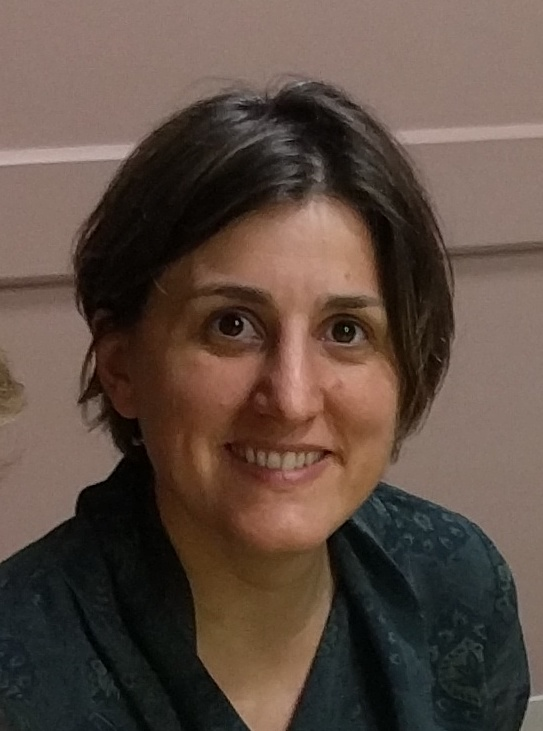
\includegraphics[width=.9\columnwidth]{cecile}
    %
    ~
    15 Avril 1983, France
    Mariée, 2 enfants
    %
    \section{Contact}
    \faEnvelope{} cecsalvato@yahoo.fr
    \faPhone{} 06 30 86 80 20
    ~
    \faHome{} 62 rue du Bourgneuf
    64160 Morlaàs
    %
%    \section{Section}
%    %
%    \section{Langues}
%    Français
%    Espagnol
    %
\end{aside}

%\section{Abs}{tract}

\setlength{\parsep}{1ex}
\setlength{\parskip}{1ex}

%----------------------------------------------------------------------------------------
%	WORK EXPERIENCE SECTION
%----------------------------------------------------------------------------------------
\vspace{7pt}
\section{Expériences }{professionnelles}
\vspace{-1ex}

\begin{entrylist}
\entry
{2020}
{Université de Pau et des Pays de l'Adour}
{Pau (64)}
{Vacataire M1 MEEF - Analyse de situation professionnelle}
%------------------------------------------------
\entry
{depuis 2013}
{Collège Joseph Peyré}
{Garlin (64)}
{\vspace{-3mm}}
%{Titulaire}
%------------------------------------------------
\entry
{2012-2013}
{Collège Jean Marie Lonne}
{Hagetmau (40)}
{\vspace{-3mm}}
%{Titulaire sur Zone de Remplacement, Landes}
%------------------------------------------------
\entry
{2010-2012}
{Lycée et Collège Climatique et Sportif Pierre de Coubertin}
{Font-Romeu (66)}
{\vspace{-3mm}}
%{Titulaire sur Zone de Remplacement, Prades Montpellier}
%------------------------------------------------
\entry
{2009-2010}
{Collège Juliette Adam}
{Gif-Sur-Yvette (91)}
{\vspace{-3mm}}
%------------------------------------------------
\entry
{2008-2009}
{Lycée de la vallée de Chevreuse}
{Gif-Sur-Yvette (91)}
{\vspace{-3mm}}
%------------------------------------------------
\entry
{2007-2008}
{Collège Charles Gounod}
{Saint-Cloud (92)}
{Stagiaire}
\end{entrylist}


%----------------------------------------------------------------------------------------
%	WORK EXPERIENCE SECTION
%----------------------------------------------------------------------------------------
\vspace{-2ex}
\section{Projets }{éducatifs}
\vspace{-1ex}

\begin{entrylist}
\entry
{2018-2020}
{Dispositif médiation par les pairs}
{Garlin}
{Membre de l'équipe référente}
%------------------------------------------------
\entry
{2018-2019}
{Atelier scientifique escape game}
{Garlin}
{Création d'un escape game}
%------------------------------------------------
\entry
{2015-2018}
{Atelier scientifique - EXPERTS à l'école}
{Garlin}
{Recherche d'indices pour résoudre des enquêtes en collaboration avec la gendarmerie de Garlin, Sciences à l'école et l'Université de Pau et des Pays de l'Adour}
%{Prêt de matériel de recherche criminelle par Sciences à l'école\\
%Collaboration avec la gendarmerie de Garlin et l'Université de Pau et des Pays de %l'Adour}
%------------------------------------------------
\entry
{2009-2010}
{Atelier scientifique - Chimie amusante}
{Gif-Sur-Yvette}
{}
%------------------------------------------------
\end{entrylist}
%------------------------------------------------

%----------------------------------------------------------------------------------------
%	Formation Pro
%----------------------------------------------------------------------------------------
\vspace{-3ex}
\section{Formations}{ professionnelles}
\vspace{-1ex}

\begin{tabular}{lp{11cm}}
    2019--2020 & %
        \vspace{-8pt}
        \begin{itemize}
            \item Sécurité au laboratoire
            \item Liaison Collège-Lycée
        \end{itemize} \vspace{-9pt} \\
    2018--2019 & %
        \vspace{-8pt}
        \begin{itemize}
            \item Formation à la médiation par les paris
            \item Créer un escape game scientifique
            \item Tablettes et démarches pédagogiques
            \item Accompagnement d'élèves en difficultés
            \item Sciences cognitives-apprentissages scolaires
        \end{itemize}\vspace{-9pt}\\
    2017--2018 & %
        \vspace{-8pt}
        \begin{itemize}
            \item La différenciation en physique-chimie
            \item L'enseignement des sciences et de la technologie en 6ème
            \item Apport des neurosciences en pédagogie
            \item De la tâche simple à la tâche complexe
        \end{itemize} \vspace{-9pt} \\
    2016--2017 & %
        \vspace{-8pt}
        \begin{itemize}
            \item Session cycle 3
            %\item Réforme du collège en sciences physiques
        \end{itemize} \vspace{-9pt} \\
    2015--2016 & %
        \vspace{-8pt}
        \begin{itemize}
            \item Mesure de la qualité de l'air, effets sur la santé et l'environnement
            %\item Réforme du collège en sciences physiques
            %\item Plan du numérique Pyrénées Atlantiques
            \item Stage "EXPERTS à l'école" à l'IRCGN
        \end{itemize} \\
\end{tabular}


%----------------------------------------------------------------------------------------
%	EDUCATION SECTION
%----------------------------------------------------------------------------------------
\vspace{-2ex}
\section{Formation}{ initiale}
\vspace{-1ex}

\begin{entrylist}
\entry
{2006-2007}
{Préparation à l'agrégation de chimie (admissible)}
{ENS Ulm}
{\vspace{-3mm}}
%------------------------------------------------
\entry
{2006}
{Professeur certifié de sciences physiques et chimiques}
{}
{\vspace{-3mm}}
%------------------------------------------------
\entry
{2005-2006}
{Préparation à l'agrégation de chimie (admissible)}
{ENS Cachan}
{\vspace{-3mm}}
%------------------------------------------------
\entry
{2003-2005}
{Magistère de Physico-Chimie Moléculaire}
{Université Paris-Sud 11 -- ENS Cachan}
{\vspace{-3mm}}
%------------------------------------------------
\entry
{2004-2005}
{Maîtrise de Chimie-Physique}
{Université Paris-Sud 11}
{\small Stage de recherche : Substitution nucléophile benzylique                      
catalysée par les complexes de palladium(0) - ICMMO - Université Paris Sud 11}
%------------------------------------------------
\entry
{2003-2004}
{Licence de Chimie-physique}
{Université Paris-Sud 11}
{\small Stage de recherche : synthèse d'un dipeptide contraint capable de mimer une hélice de type polyproline II - 
Institut des Biomolécules Max Mousseron - Université Montpellier 2}
%------------------------------------------------
\entry
{2001-2003}
{Classes Préparatoires aux Grandes Écoles}
{Lycée François Arago, Perpignan}
{PCSI - PC}
\end{entrylist}

%----------------------------------------------------------------------------------------
%	INTERESTS SECTION
%----------------------------------------------------------------------------------------
% \section{interests}
%   \vspace{-0.2cm}
%
% \textbf{professional:} professional interest 1, professional interest 2 and professional interest 3.
% \textbf{personal:} personal interest 1, personal interest 2, personal interest 3 and personal interest 4.
%----------------------------------------------------------------------------------------

\end{document}
